\documentclass{beamer}

\usepackage{pgfpages}
%\setbeameroption{show notes on second screen}

\usetheme{CambridgeUS}
\usecolortheme{dolphin}
\usefonttheme{serif}

\definecolor{rit@orange}{HTML}{F36E21}
\definecolor{rit@brown}{HTML}{513127}
\setbeamercolor{structure}{fg=rit@orange}
\setbeamercolor{palette primary}{fg=white, bg=rit@brown}
\setbeamercolor{palette secondary}{fg=rit@brown}
\setbeamercolor{palette tertiary}{fg=white, bg=rit@orange}
\setbeamercolor{titlelike}{fg=rit@brown}
\setbeamercolor{normal text}{fg=rit@brown}

\setbeamertemplate{enumerate}[circle]
\setbeamertemplate{items}[circle]

\AtBeginSection{\frame{\sectionpage}}

\setbeamertemplate{section page}
{
    \begin{centering}
    \begin{beamercolorbox}[sep=12pt,center]{part title}
    \usebeamerfont{section title}\insertsection\par
    \end{beamercolorbox}
    \end{centering}
}


\beamertemplatenavigationsymbolsempty

\logo{\includegraphics[width=0.50in]{img/astlogo}}

\pdfpageattr {/Group << /S /Transparency /I true /CS /DeviceRGB>>}

\usepackage{amsmath,amssymb,commath,physics}
\usepackage{cclicenses,copyrightbox}
\usepackage{float,subcaption}
\usepackage{xcolor}


\usepackage[style=trad-plain,citestyle=authoryear,maxcitenames=3]{biblatex}
\addbibresource{bibliography.bib}


\DeclareCiteCommand{\citefirst}
  {\usebibmacro{prenote}}
  {\renewbibmacro*{name:andothers}{}%
   \usebibmacro{citeindex}%
   \usebibmacro{cite}}
  {\multicitedelim}
  {\usebibmacro{postnote}}





\usepackage{animate}


\DeclareMathOperator*{\argmin}{argmin}

\usepackage{tikz}
\usetikzlibrary{arrows,shapes,positioning,shadows,trees}

\tikzset{
basic/.style   = {draw, text width=2cm, drop shadow, font=\sffamily, rectangle},
root/.style    = {basic, rounded corners=2pt, thin, align=center,
                  fill=green!60},
level 1/.style = {sibling distance=40mm},
level 2/.style = {basic, rounded corners=6pt, thin, align=center, fill=green!30,
                  text width=8em},
level 3/.style = {basic, thin, align=left, fill=white}
}



\newcommand{\variablestarclasses}{
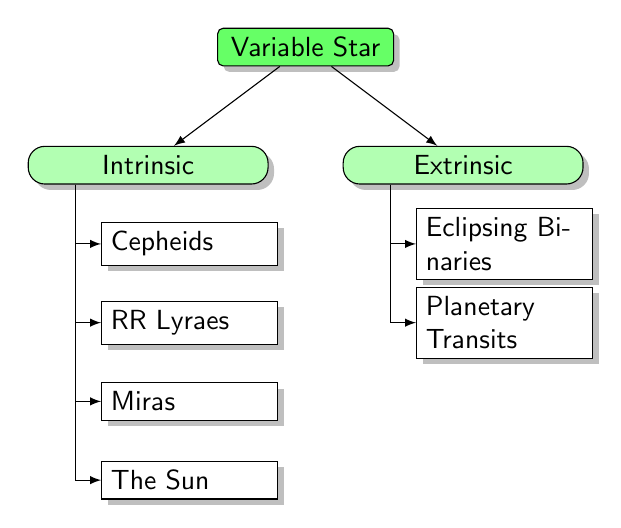
\begin{tikzpicture}[edge from parent/.style = {->,draw}, >=latex]
  \node[root]{Variable Star}
    child {node[level 2] (Intrinsic) {Intrinsic}}
    child {node[level 2] (Extrinsic) {Extrinsic}}
  ;

  \begin{scope}[every node/.style={level 3}]
    %% Intrinsic %%
    \node [below of = Intrinsic, xshift=15pt]
          (Cepheids)
          {Cepheids};

    \node [below of = Cepheids]
          (RR Lyraes)
          {RR Lyraes};

    \node [below of = RR Lyraes]
          (Miras)
          {Miras};

    \node [below of = Miras]
          (The Sun)
          {The Sun};

    %% Apparent %%
    \node [below of = Extrinsic, xshift=15pt]
          (Eclipsing Binaries)
          {Eclipsing Binaries};

    \node [below of = Eclipsing Binaries]
          (Planetary Transits)
          {Planetary Transits};
  \end{scope}

  \foreach \value in {Cepheids,RR Lyraes,Miras,The Sun}
    \draw[->] (Intrinsic.195) |- (\value.west);

  \foreach \value in {Eclipsing Binaries,Planetary Transits}
    \draw[->] (Extrinsic.195) |- (\value.west);

\end{tikzpicture}
}

\newcommand{\trigonometry}{
\begin{tikzpicture}[scale=5,cap=round]
  \def\costhirty{0.8660256}

  \draw[red,thick]
    (3mm,0pt) arc(0:30:3mm);

  \draw
    (15:2mm) node {$\Phi_k$};

  \draw
    (30:1cm) -- node[right=1pt] {$b_k$}
   +(0,-.5);

  \draw
    (0,0) -- node[below=2pt] {$a_k$}
    (\costhirty,0);

  % \draw[black] (1,0) --
  %   node [right=1pt,fill=white]
  %   {
  %     $\displaystyle \tan \alpha \color{black}=
  %     \frac{{\color{black}\sin \alpha}}{\color{black}\cos \alpha}$
  %   } (intersection of 0,0--30:1cm and 1,0--1,1) coordinate (t);

  \draw
    (0,0) -- node[above=2pt] {$A_k$}
    (intersection of 0,0--30:1cm and \costhirty,0--\costhirty,1);
\end{tikzpicture}
}



\title[Variable Stars]{
  Fourier decomposition of variable stars using regularized regression
}

\author[Daniel Wysocki]{
  Daniel Wysocki
}

\institute[RIT]{
  Rochester Institute of Technology
}


\date[Dec 7, 2015]{AST Graduate Seminar -- December 7th, 2015}


\begin{document}

\maketitle

\section{Variable Stars}

\begin{frame}{Overview}
  \begin{itemize}
  \item in general, any star whose brightness changes on short timescales is
    a variable star
  \item many different types exist
  \end{itemize}
\end{frame}

\begin{frame}{Some classes of variable stars}
  \begin{figure}[h]
    \centering
    \variablestarclasses
  \end{figure}
\end{frame}

\begin{frame}{Pulsating periodic intrinsic variables}

  For the remainder of this talk:
  \begin{center}
    variable star $\equiv$ pulsating periodic intrinsic variable star.
  \end{center}

  \begin{itemize}
  \item not in hydrostatic equilibrium
    \begin{itemize}
    \item typically in the instability strip
    \end{itemize}
  \item periodic oscillation
    \begin{itemize}
    \item predictable
    \end{itemize}
  \item stellar pulsation
    \begin{itemize}
    \item $\kappa$-mechanism
    \end{itemize}
  \end{itemize}
\end{frame}

\begin{frame}{Henrietta Swan Leavitt}
  \begin{figure}[h]
    \centering
    \begin{subfigure}[c]{0.3\textwidth}
      \centering
        \copyrightbox[r]{
          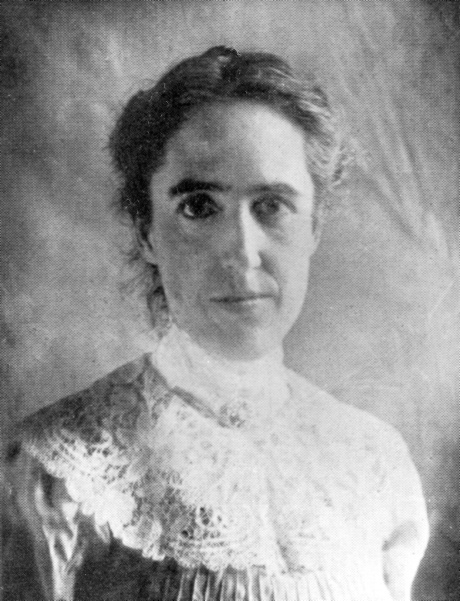
\includegraphics[width=0.98\textwidth]{img/leavitt-photo}
        }{
          Public domain in USA
        }
      \caption*{Henrietta Swan Leavitt}
    \end{subfigure}
    \begin{subfigure}[c]{0.65\textwidth}
      \begin{itemize}
      \item worked as a ``computer'' at Harvard in the early 20th century
      \item discovered a relation between the period and luminosity
        of Cepheids
        \begin{itemize}
        \item Leavitt's law
        \item standard candles
        \end{itemize}
      \item enabled Edwin Hubble to measure the expansion of the Universe
      \end{itemize}
    \end{subfigure}
  \end{figure}
\end{frame}


\section{Light Curves}

\begin{frame}{Overview}
  \begin{itemize}
  \item repeated photometric measurements of an object over time
  \item plotting brightness versus time gives us a light curve
  \end{itemize}
\end{frame}

\begin{frame}{Light Curve of a Cepheid variable star}
  \begin{figure}[h]
    \centering
    \copyrightbox{
      \animategraphics[loop,height=0.75\textheight,autoplay]
        {60}{img/simulation/OGLE-LMC-CEP-0002-simulation-}{00}{99}
    }{
      \cc Daniel Wysocki
    }
    \caption*{Visualization of OGLE-LMC-CEP-0002}
  \end{figure}
\end{frame}

\begin{frame}{Fourier decomposition}
  \begin{figure}
    \centering
    \begin{subfigure}[c]{0.3\textwidth}
      \centering
        \copyrightbox[r]{
          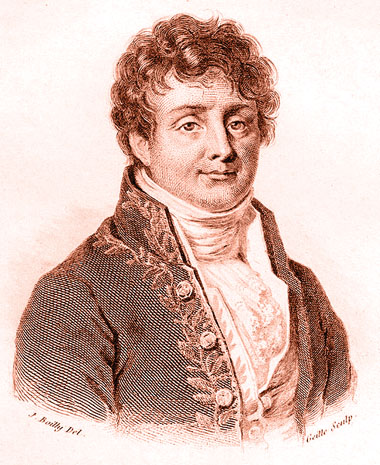
\includegraphics[width=0.98\textwidth]{img/joseph-fourier}
        }{
          Public domain in USA
        }
      \caption*{Joseph Fourier}
    \end{subfigure}
    \begin{subfigure}[c]{0.65\textwidth}
      \begin{itemize}
      \item any continuous, periodic function can be represented as an
        infinite Fourier series
        \begin{displaymath}
          f(t) = A_0 + \sum_{k=1}^\infty A_k \cos(k \omega t + \Phi_k)
        \end{displaymath}
      \item characterized by the angular frequency $\omega$, the mean $A_0$,
        the amplitudes $A_k$, and the phase shifts $\Phi_k$
      \end{itemize}
    \end{subfigure}

    \textcite{fourier1808memoire}
  \end{figure}
\end{frame}

\begin{frame}{Fourier decomposition of periodic light curves}
  \begin{displaymath}
    m(t) = A_0 + \sum_{k=1}^n A_k \cos(k \omega t + \Phi_k)
  \end{displaymath}
  \begin{itemize}
  \item Cepheid-like light curves well described by $n$th order Fourier Series
  \item physically they are close to harmonic oscillators
  \end{itemize}
\end{frame}

\begin{frame}{Solving for series parameters}
  \begin{align*}
    m(t) &=
    A_0 +
    \sum_{k=1}^n A_k \cos(k {\color{red} \omega} t + {\color{red} \Phi_k})
    \\ &=
    A_0 +
    \sum_{k=1}^n [
      a_k \sin(k {\color{red} \omega} t) +
      b_k \cos(k {\color{red} \omega} t)
    ]
  \end{align*}
  \begin{itemize}
  \item Fourier series are non-linear
  \item simultaneously finding the optimal $n$, $\omega$, $A_k$, and $\Phi_k$
    is not easy
  \end{itemize}
\end{frame}

\begin{frame}{Period finding}
  \begin{itemize}
  \item the most important parameter is the period
    \begin{displaymath}
      \omega = 2\pi/P
    \end{displaymath}
  \item we can approximate this by itself using a periodogram
    \begin{itemize}
    \item Lomb-Scargle
    \end{itemize}
  \end{itemize}
\end{frame}

\begin{frame}{Lomb-Scargle periodogram}
  \begin{figure}[ht]
    \centering
    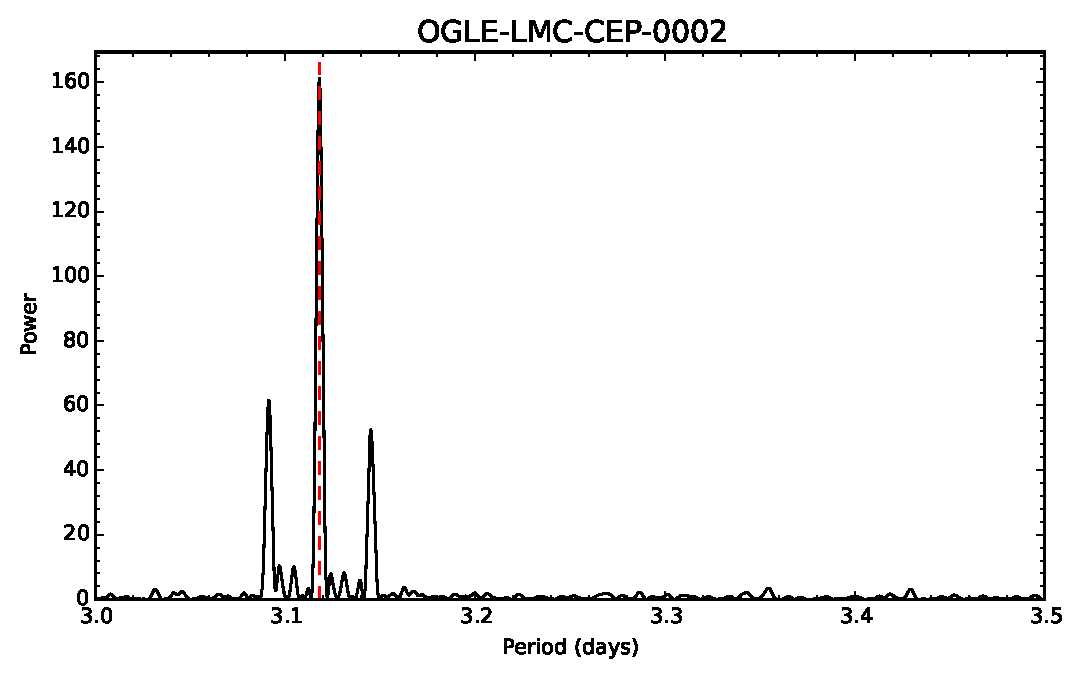
\includegraphics[width=0.75\textwidth]{img/periodogram}
    \caption*{Periodogram of star with $3.11804$ day period}
  \end{figure}
\end{frame}


\begin{frame}{It's linear!}
  \begin{displaymath}
    m(t) =
    A_0 +
    \sum_{k=1}^n \qty[
      a_k \sin(k {\color{blue} \omega} t) +
      b_k \cos(k {\color{blue} \omega} t)
    ]
  \end{displaymath}
  \begin{center}
    can be written in the form
  \end{center}
  \begin{displaymath}
    \vb{X} \vec\beta = \vec{y}
  \end{displaymath}
  \begin{center}
    which can be approximated using ordinary linear regression
  \end{center}
\end{frame}

\begin{frame}{System of equations}
  \begin{gather*}
    \vec{y} \to \mqty(m_1 & m_2 & \ldots & m_N)
    \\
    \vec\beta \to \mqty(A_0 & a_1 & b_1 & \ldots & a_n & b_n)
    \\
    \vb{X} \to \mqty(
      1 & \sin(1 \omega t_1) & \cos(1 \omega t_1) & \ldots &
          \sin(n \omega t_1) & \cos(n \omega t_1)
      \\
      \vdots & \vdots & \vdots & \ddots & \vdots & \vdots
      \\
      1 & \sin(1 \omega t_N) & \cos(1 \omega t_N) & \ldots &
          \sin(n \omega t_N) & \cos(n \omega t_N)
    )
  \end{gather*}
\end{frame}

\begin{frame}{How many terms?}
  \begin{itemize}
  \item wait, we never decided on the order of the fit, $n$
  \item it's just a truncated series expansion
    \begin{itemize}
    \item more terms means better, right?
    \item let's try 100 terms\ldots
    \end{itemize}
  \end{itemize}
\end{frame}

\begin{frame}{Overfitting}
  \begin{figure}[h]
    \centering
    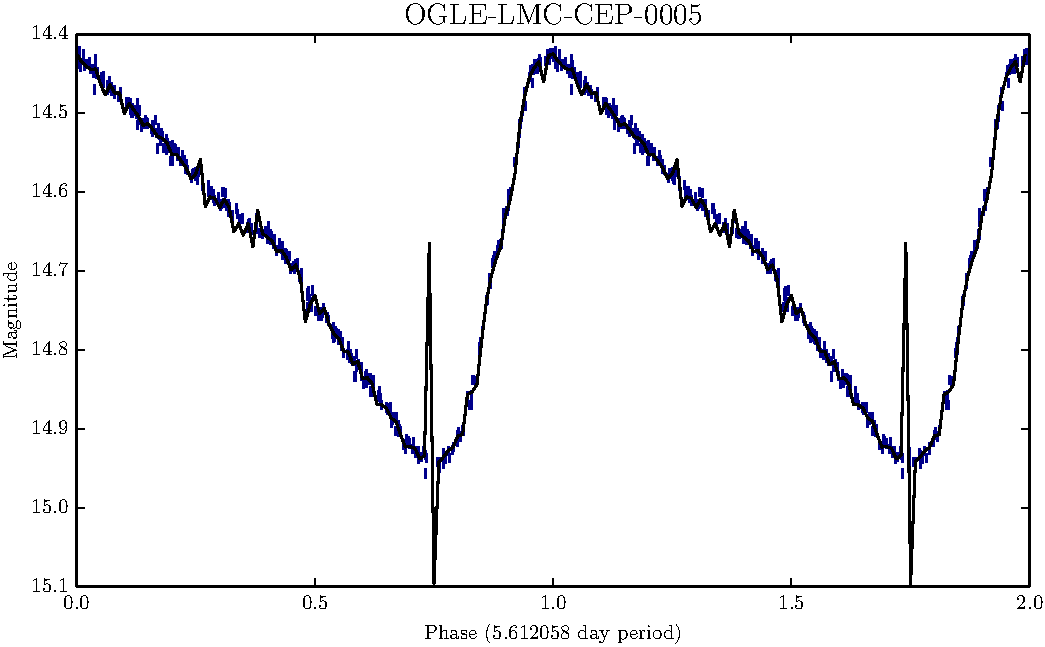
\includegraphics[width=0.75\textwidth]{img/fits/OGLE-LMC-CEP-0005-degree100}
    \caption*{$100$th order fit}
  \end{figure}
\end{frame}

\begin{frame}{Overfitting (again)}
  \begin{figure}[h]
    \centering
    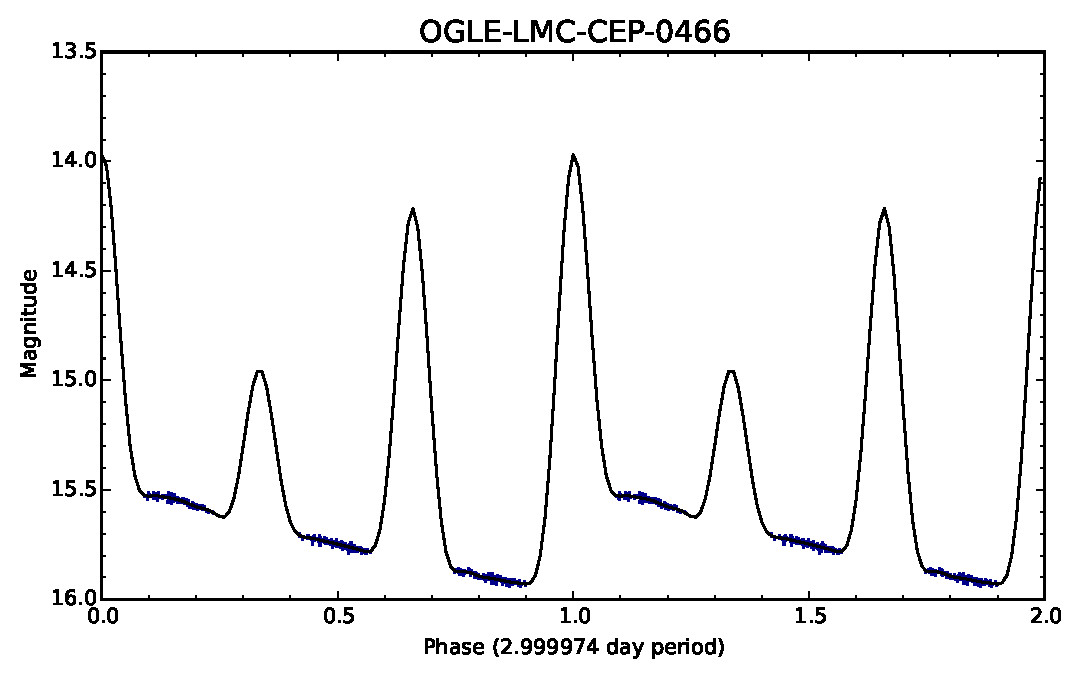
\includegraphics[width=0.75\textwidth]{img/lightcurve-overfit}
    \caption*{$12$th order fit}
  \end{figure}
\end{frame}

\begin{frame}{Underfitting}
  \begin{figure}[h]
    \centering
    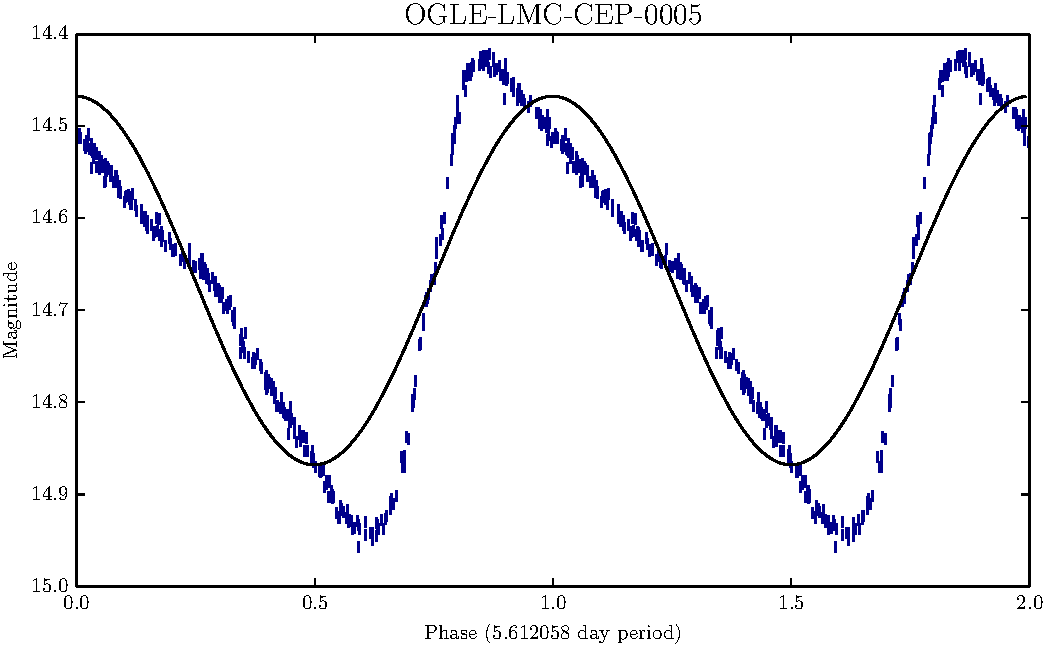
\includegraphics[width=0.75\textwidth]{img/fits/OGLE-LMC-CEP-0005-degree2}
    \caption*{$1$st order fit}
  \end{figure}
\end{frame}

\begin{frame}{Choosing $n$}
  \begin{itemize}
  \item need some criteria to decide the order of the fit
  \item Baart's criteria is often used for this
    \begin{itemize}
    \item iterative approach, increasing $n$ until diminishing returns
    \item good at avoiding underfitting
    \item bad at avoiding overfitting
    \end{itemize}
  \end{itemize}
\end{frame}

\begin{frame}{Taking a step back}
  \begin{itemize}
  \item take photometric measurements
  \item \only<1>{find the period}
        \only<2>{\textbf{periodogram}}
  \item \only<1>{approximate coefficients with OLS}
        \only<2>{\textbf{regression}}
  \item \only<1>{find the best order of fit using Baart's criteria}
        \only<2>{\textbf{model selection}}
  \end{itemize}
\end{frame}

\begin{frame}{Plotypus}
\begin{figure}
  \centering
  \begin{subfigure}[c]{0.2\textwidth}
    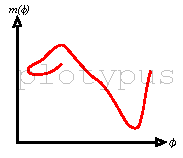
\includegraphics[width=\textwidth]{img/plotypus}

    
\includegraphics[width=\textwidth]{img/plotypus-qr}
  \end{subfigure}
  \begin{subfigure}[c]{0.7\textwidth}
    \begin{itemize}
      \item tool for modeling and plotting light curves
      \item free and open source
      \item version controlled and documented
      \item generated the light curve plots in this presentation
      \item \href{https://astroswego.github.io/plotypus/}
                 {astroswego.github.io/plotypus/}
      \item download today!
    \end{itemize}
  \end{subfigure}

  \textcite{plotypus2015}
\end{figure}
\end{frame}

\begin{frame}{Unconstrained regression}
  \begin{displaymath}
    \vb{X} \vec\beta = \vec{y}
  \end{displaymath}
  \begin{align*}
    (A_0, a_k, b_k) &=
    \argmin_\beta \norm{\vb{X} \vec\beta - \vec{y}}_2^2
    \\ &=
    \argmin_{(A_0, a_k, b_k)}
    \sum_{i=1}^N \qty(
      A_0 +
      \sum_{k=1}^n \qty[
        \begin{aligned}
           & a_k \sin(k \omega t_i)
          \\
          +& b_k \cos(k \omega t_i)
        \end{aligned}
      ] - m_i
    )^2
  \end{align*}
  \begin{center}
    Find coefficients which minimize magnitude of residual vector
  \end{center}
\end{frame}


\begin{frame}{$\ell_0$ regularization}
  \begin{displaymath}
    (A_0, a_k, b_k) =
    \argmin_\beta \qty{
      \norm{\vb{X} \vec\beta - \vec{y}}_2^2 +
      \lambda \norm{\vec\beta}_0
    }
  \end{displaymath}
  \begin{itemize}
  \item $\norm{\vec\beta}_0$ is equal to the number of non-zero terms in $\vec\beta$
  \item adds a penalty on the number of parameters, weighted by $\lambda$
  \item this is computationally expensive
  \end{itemize}
\end{frame}


\begin{frame}{$\ell_1$ regularization (LASSO)}
  \begin{align*}
    (A_0, a_k, b_k) &=
    \argmin_\beta \qty{
      \norm{\vb{X} \vec\beta - \vec{y}}_2^2 +
      \norm{\vec\beta}_1
    }
    \\ &=
    \argmin_{(A_0, a_k, b_k)} \qty{
    \begin{aligned}
    &\sum_{i=1}^N \qty(
      A_0 +
      \sum_{k=1}^n \qty[
        \begin{aligned}
           & a_k \sin(k \omega t_i)
          \\
          +& b_k \cos(k \omega t_i)
        \end{aligned}
      ] - m_i
    )^2
    \\ +&
    \lambda \sum_{k=0}^n \qty( \abs{a_k} + \abs{b_k} )
    \end{aligned}
    }
  \end{align*}
  \begin{itemize}
  \item least absolute shrinkage and selection operator (LASSO)
  \item adds a penalty on the sum of the amplitudes, weighted by $\lambda$
  \item automatically zeroes out non-contributing terms
  \end{itemize}
\end{frame}

\begin{frame}{Model selection with grid search}
  \begin{itemize}
  \item use grid search with cross-validation
    \begin{itemize}
    \item search over the order of fit $n$
    \end{itemize}
  \item cross-validation helps fit underlying function, not just the data
  \end{itemize}
\end{frame}

\section{Results}

\begin{frame}{OLS/Baart light curve}
  \begin{figure}[ht]
    \centering
    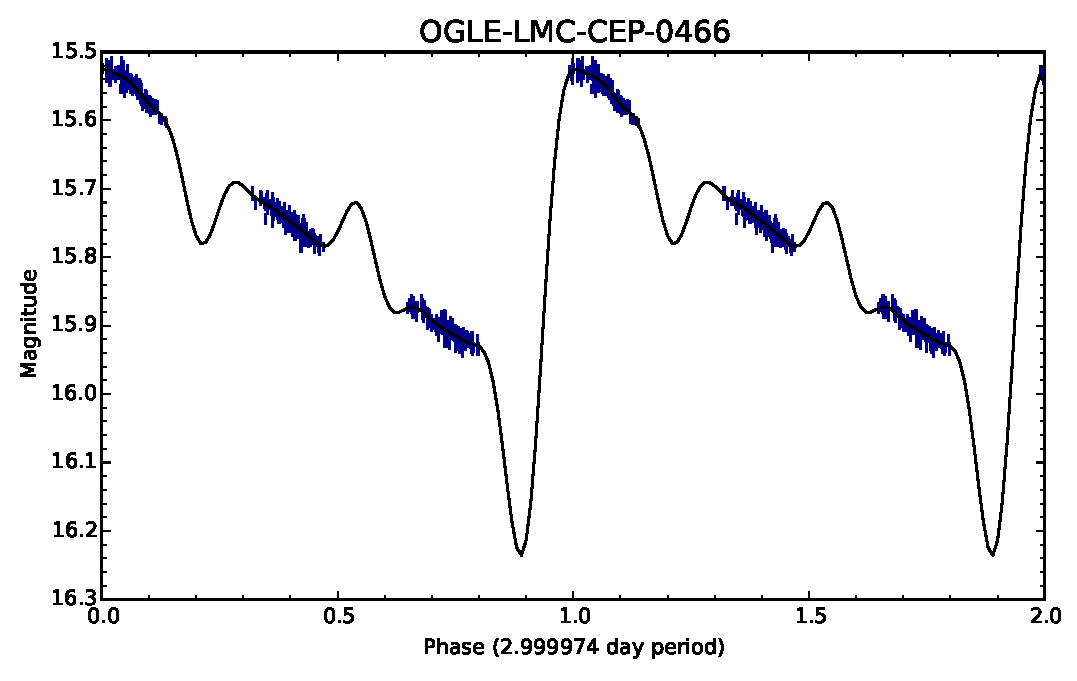
\includegraphics[width=0.75\textwidth]{img/lightcurve-ols}
    \caption*{$10$th order fit using OLS/Baart.}
  \end{figure}
\end{frame}

\begin{frame}{LASSO light curve}
  \begin{figure}[ht]
    \centering
    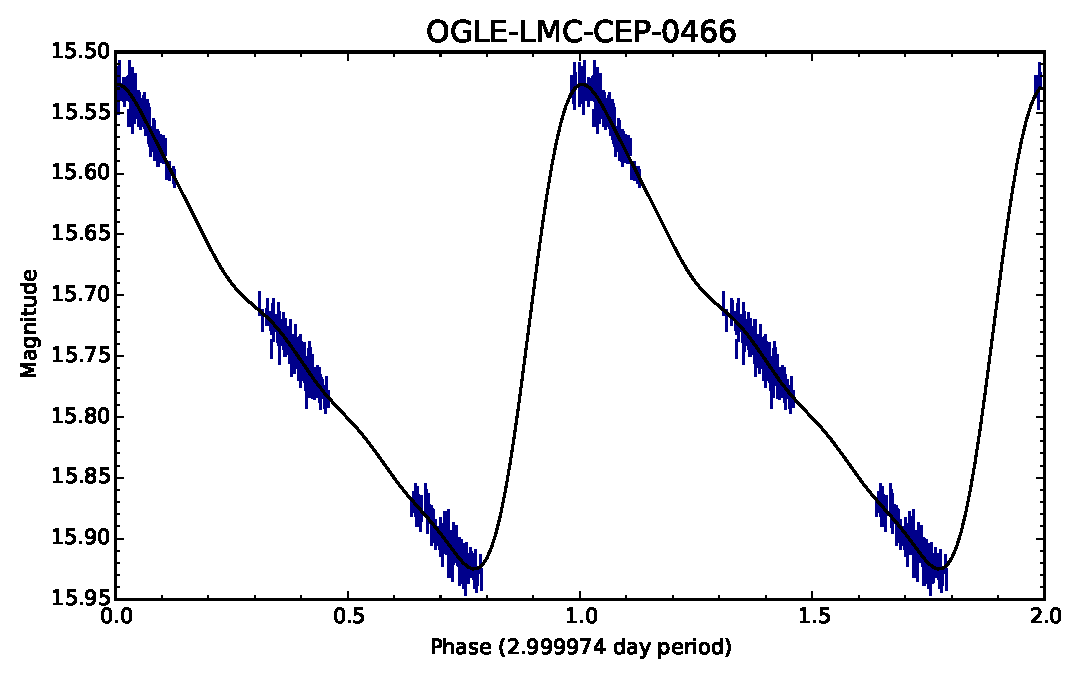
\includegraphics[width=0.75\textwidth]{img/lightcurve-lasso}
    \caption*{$10$th order fit using Lasso/Grid Search.}
  \end{figure}
\end{frame}


\begin{frame}{Performance of LASSO/grid search versus OLS/Baart}
  \begin{table}[ht]
  \tiny
  \begin{tabular}{ c c c c c c c }
    Galaxy & Type & Stars & N (SD) & LASSO $R^2$ (MAD) & Baart $R^2$ (MAD) & Significance \\ \hline
    (all) & (all) & 52844 & 643.1 (462.0) & \textbf{ 0.8594 (0.1741)} &  0.8492 (0.1864) & $p < .0001$ \\
    (all) & CEP & 7999 & 740.1 (298.4) & \textbf{ 0.9816 (0.0191)} &  0.9810 (0.0198) & $p < .0001$ \\
    (all) & T2CEP & 596 & 747.6 (612.0) & \textbf{ 0.9145 (0.1159)} &  0.9009 (0.1328) & $p < .0001$ \\
    (all) & ACEP & 89 & 497.3 (225.0) & \textbf{ 0.9700 (0.0245)} &  0.9689 (0.0267) & $p < .0001$ \\
    (all) & RRLYR & 44160 & 624.4 (481.6) & \textbf{ 0.8316 (0.1816)} &  0.8197 (0.1926) & $p < .0001$ \\
    LMC & (all) & 28491 & 522.3 (227.7) & \textbf{ 0.7812 (0.1695)} &  0.7723 (0.1779) & $p < .0001$ \\
    LMC & CEP & 3342 & 536.8 (219.7) & \textbf{ 0.9840 (0.0172)} &  0.9833 (0.0180) & $p < .0001$ \\
    LMC & T2CEP & 201 & 538.3 (232.6) & \textbf{ 0.8672 (0.1569)} &  0.8599 (0.1653) & $p < .0001$ \\
    LMC & ACEP & 83 & 477.3 (214.7) & \textbf{ 0.9704 (0.0233)} &  0.9701 (0.0245) & $p < .0001$ \\
    LMC & RRLYR & 24865 & 520.3 (228.6) & \textbf{ 0.7544 (0.1667)} &  0.7452 (0.1755) & $p < .0001$ \\
    SMC & (all) & 7146 & 851.4 (256.7) & \textbf{ 0.9109 (0.1241)} &  0.9091 (0.1266) & $p < .0001$ \\
    SMC & CEP & 4625 & 886.5 (256.2) & \textbf{ 0.9800 (0.0195)} &  0.9796 (0.0200) & $p < .0001$ \\
    SMC & T2CEP & 42 & 891.2 (241.4) & \textbf{ 0.7965 (0.2235)} &  0.7888 (0.2379) & $p < .0001$ \\
    SMC & ACEP & 6 & 774.3 (190.2) &  0.9277 (0.0709) &  0.9272 (0.0706) & $p = 0.2188 $ \\
    SMC & RRLYR & 2473 & 785.2 (244.8) & \textbf{ 0.6299 (0.1915)} &  0.6203 (0.1962) & $p < .0001$ \\
    BLG & (all) & 17207 & 756.8 (698.1) & \textbf{ 0.9579 (0.0445)} &  0.9527 (0.0514) & $p < .0001$ \\
    BLG & CEP & 32 & 824.2 (569.0) & \textbf{ 0.9742 (0.0342)} &  0.9703 (0.0396) & $p < .0001$ \\
    BLG & T2CEP & 353 & 849.7 (746.8) & \textbf{ 0.9525 (0.0643)} &  0.9457 (0.0747) & $p < .0001$ \\
    BLG & RRLYR & 16822 & 754.7 (697.2) & \textbf{ 0.9581 (0.0440)} &  0.9528 (0.0509) & $p < .0001$ \\ \hline
  \end{tabular}
  \captionsetup{width=0.8\textwidth}
  \caption*{\tiny Median coefficients of determination ($R^2$) and median absolute deviations (MAD) for models selected by cross-validated LASSO and Baart's ordinary least squares on OGLE $I$-band photometry. P-values obtained by paired Mann-Whitney $U$ tests.}
  \end{table}
\end{frame}


\begin{frame}{Missing harmonics}
  \begin{itemize}
  \item LASSO makes no distinction between higher and lower order terms
    \begin{itemize}
    \item if it doesn't contribute, it goes to zero
    \end{itemize}
  \item this can result in $A_i = 0$, when $A_j \neq 0$, $j > i$
    \begin{itemize}
    \item contrary to pulsation models, which say amplitude decreases with order
      \begin{displaymath}
        A_1 > A_2 > \ldots > A_n
      \end{displaymath}
    \end{itemize}
  \item explanations:
    \begin{itemize}
    \item harmonics absent from observations
      \begin{itemize}
      \item e.g. we observe only near zero-crossing
      \end{itemize}
    \item interference pattern in pulsation (gets political)
    \item others? (please tell me)
    \end{itemize}
  \end{itemize}
\end{frame}

\begin{frame}{Multifrequency variable stars}
  \begin{gather*}
    m(t) =
    A_0 +
    \sum_{k_1=-n}^n \ldots \sum_{k_p=-n}^n
    A_{\vb{k}} \cos((\vb{k} \cdot \boldsymbol\omega) t + \Phi_{\vb{k}})
    \\
    \vb{k} \to \mqty( k_1 & \ldots & k_p )
    \quad
    \boldsymbol\omega \to \mqty( \omega_1 & \ldots & \omega_p )
  \end{gather*}
  \begin{itemize}
  \item some variable stars oscillate with multiple ($p$) periods
  \item OLS fails to accurately fit these light curves
    \begin{itemize}
    \item tools exist to manually fix certain amplitudes to zero
    \end{itemize}
  \item LASSO successful in automatically zeroing out amplitudes
  \end{itemize}

  \centering
  \textcite{2015arXiv151200004B}
\end{frame}

\section{References}

\begin{frame}[allowframebreaks]

\printbibliography[heading=subbibliography]

\end{frame}

\end{document}
